\section{The Electric Field Near a Charged Rod}

\begin{comment}
This "lab" is by Matt Trawick.  I used this in my class for several years from an MS word file.  I converted it to latex and added it to the lab manual in 2015.  The figures could still be cleaned up a bit, but they work.
... and now I've cleaned up the figures too.
\end{comment}

\makelabheader %(Space for student name, etc., defined in master.tex)

\begin{wrapfigure}[10]{r}{0.385\textwidth}
\vspace{-.25in}
    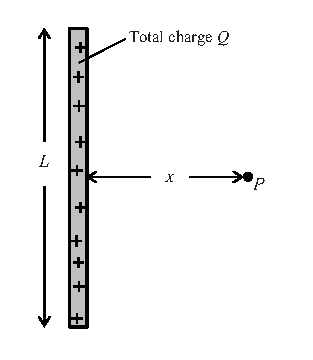
\includegraphics[width=0.3\textwidth]{electric_field_near_a_charged_rod/fig1.eps}
\end{wrapfigure}

\vspace{1cm}

\textbf{Objective and statement of the problem:}

Calculate the electric field $\vec{E}$ at a point $P$ a distance $x$ away from the midpoint of a thin rod
of length $L$ and total charge $Q$.

\vspace{1cm}

\textbf{Introduction and outline of solution:}

Think of the rod as a bunch of teeny-tiny little point charges $dQ$ arranged in a row. You will solve this problem by calculating the sum (actually an integral) of the electric fields due to each point charge.  In the second figure, below, we have added a set of coordinate axes, and defined a tiny bit of charge $dQ$ that is on a tiny bit of length $dy$.  
\par

\begin{wrapfigure}[6]{r}{0.4\textwidth}
%\vspace{-23pt}
\vspace{-.65in}
   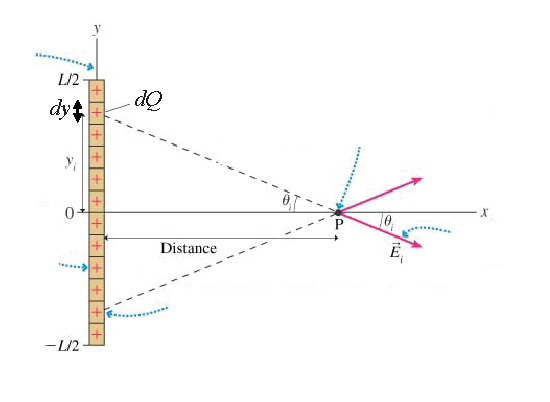
\includegraphics[width=0.4\textwidth]{electric_field_near_a_charged_rod/fig2.eps}
\end{wrapfigure}

%\vspace{0.1cm}
%{\centering \resizebox*{0.5\textwidth}{!}{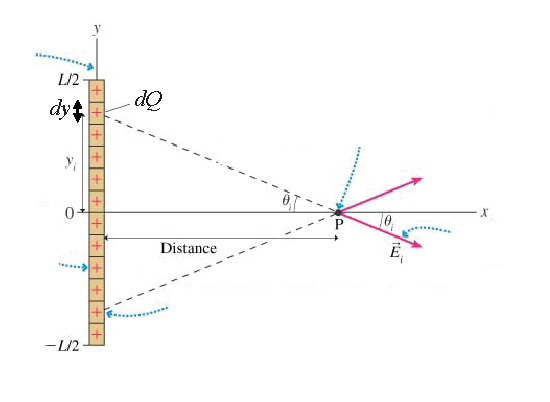
\includegraphics{electric_field_near_a_charged_rod/fig2.eps}} \par}

\par
\vspace{0.5cm}
\par
\textbf{Step 1:} \newline
In words, what is the direction of the electric field at point $P$ due to just one little bit of charge $dQ$ shown?

\vspace{.6in}

What is the direction of the electric field at point $P$ due to the whole rod?

\vspace{.6in}

\textbf{Step 2:} \newline
What is the magnitude of the electric field $|d\vec{E}|$  due to just the bit of charge $dQ$?  (Write the relevant distance in terms of $x$ and $y$, not $\theta$.)
\[
|d\vec{E}|=\hspace{0.7in}
\]
\vspace{.3in}

\textbf{Step 3:} \newline
What is the magnitude of the $x$-component of   $d\vec{E}$?  (It's similar to your answer above but with an extra $\sin \theta$ or $\cos \theta$.) 
\[
d\vec{E}_x=\hspace{1in}
\]
\vspace{.3in}

\pagebreak
\textbf{Step 4:} \newline
Rewrite the last step, giving  $\sin \theta$ or $\cos \theta$ in terms of a ratio involving $x$, $y$, and/or $\sqrt{x^2 + y^2}$.
\[
d\vec{E}_x=\hspace{1in}
\]
\vspace{.3in}

\textbf{Step 5:} \newline
The linear charge density $\lambda$ of the rod is given by $\lambda = Q/L$.  Write $dQ$ in terms of $\lambda$  and $dy$, then in terms of $Q$, $L$ and $dy$.
\[
dQ=\hspace{0.7in}=\hspace{0.7in}
\]
\vspace{.3in}

\textbf{Step 6:} \newline
Combine your answers to steps 4 and 5 to write $\vec{E}$ as a single integral over $dy$ which you can solve.  What are the limits of the integral?
\[
\vec{E}=\int d\vec{E}_x=\hspace{1.5in}
\]
\vspace{.3in}

\textbf{Step 7:} \newline
Evaluate the integral.  
\[
\vec{E}=\hspace{2in}
\]

 \vspace{3in}

\textit{Note: one of the following might be helpful:}
\begin{flalign*}
& \int \! \frac{1}{\left (u^2 + a^2 \right )^\frac{3}{2}} \, du=\frac{u}{a^2 \sqrt{u^2 + a^2}} &\\
& \int \! \frac{u}{\left (u^2 + a^2 \right )^\frac{3}{2}} \, du=\frac{-1}{\sqrt{u^2 + a^2}} \\
& \int \! \frac{1}{u^2 + a^2} \, du=\frac{1}{a} \tan^{-1} \frac{u}{a}
\end{flalign*}
%\]

